
\documentclass[xetex,professionalfont]{beamer}

\usepackage{amsmath}

\usepackage{mathtools}

\usepackage{amssymb}

\usepackage{xspace}

\usepackage{booktabs}


\usepackage{fontspec}
\setmonofont[Scale=0.7]{Droid Sans Mono} %

\usepackage[caption=false]{subfig}
\captionsetup{belowskip=0pt,aboveskip=0pt}

\usepackage{csquotes}

\usepackage{copyrightbox}

\usepackage[english]{babel}


\usepackage{tikz}

\usepackage{pgfplots}

\usetikzlibrary{backgrounds,arrows,automata}

\definecolor{xblue}{RGB}{210,224,255}
\definecolor{xyellow}{RGB}{255,255,205}
\definecolor{xred}{RGB}{255,205,205}
\definecolor{xgreen}{RGB}{205,255,205}


\hypersetup{pdftitle={DLVC Lecture 6},pdfsubject={},pdfauthor={Christopher Pramerdorfer},colorlinks,urlcolor=tuwcvl_cvl_blue,linkcolor=tuwcvl_textlight,citecolor=tuwcvl_textlight}

\makeatletter\renewcommand{\CRB@setcopyrightfont}{\tiny\color{lightgray}}

\let\oldemph\emph
\renewcommand\emph[1]{\textcolor{tuwcvl_cvl_blue}{#1}}

\usefonttheme[onlymath]{serif}

\usetheme{dlvc}


\definecolor{dred}{rgb}{0.85,0,0.1}
\definecolor{dgreen}{rgb}{0,0.85,0.1}
\definecolor{dblue}{rgb}{0,0.1,0.85}


\newcommand{\ie}{\mbox{i.e.}\xspace} %
\newcommand{\eg}{\mbox{e.g.}\xspace} %

\DeclareMathOperator*{\argmin}{arg\,min}
\DeclareMathOperator*{\argmax}{arg\,max}

\newcommand{\NN}{\mathbb{N}}
\newcommand{\ZZ}{\mathbb{Z}}
\newcommand{\QQ}{\mathbb{Q}}
\newcommand{\RR}{\mathbb{R}}

\renewcommand{\vec}[1]{\ensuremath{\mathbf{#1}}}

\newcommand{\va}{\vec{a}}
\newcommand{\vb}{\vec{b}}
\newcommand{\vc}{\vec{c}}
\newcommand{\ve}{\vec{e}}
\newcommand{\vr}{\vec{r}}
\newcommand{\vs}{\vec{s}}
\newcommand{\vt}{\vec{t}}
\newcommand{\vu}{\vec{u}}
\newcommand{\vv}{\vec{v}}
\newcommand{\vw}{\vec{w}}
\newcommand{\vx}{\vec{x}}
\newcommand{\vy}{\vec{y}}
\newcommand{\vz}{\vec{z}}
\newcommand{\vo}{\vec{o}}
\newcommand{\vm}{\vec{m}}
\newcommand{\vn}{\vec{n}}

\makeatletter
\let\@@magyar@captionfix\relax
\makeatother

\newcommand{\vA}{\vec{A}}
\newcommand{\vW}{\vec{W}}
\newcommand{\vX}{\vec{X}}
\newcommand{\bth}{\boldsymbol{\theta}}
\newcommand{\cD}{\mathcal{D}}

\DeclareMathOperator*{\sgn}{sgn}
\DeclareMathOperator*{\mean}{mean}

\makeatletter
\def\verbatim@font{\linespread{1}\normalfont\ttfamily}
\makeatother


\title{Deep Learning for Visual Computing}
\subtitle{Modern Classification Networks}
\author{Christopher Pramerdorfer}
\institute{Computer Vision Lab, TU Wien}

\begin{document}


\begin{frame}
	\maketitle
\end{frame}


\begin{frame}
	\frametitle{Topics}

	Optimization vs.~Machine Learning
	\begin{itemize}
		\item Regularization
	\end{itemize}

	\bigskip

	Modern classification networks
	\begin{itemize}
		\item Residual networks
		\item Efficient architectures
	\end{itemize}

	\bigskip

	Pushing classification performance
	\begin{itemize}
		\item Fine-tuning
		\item Handling imbalanced data
	\end{itemize}

\end{frame}


\begin{frame}
	\frametitle{Optimization vs.~Machine Learning}
	\framesubtitle{Regularization}

	Recall from last lecture that our goal is to
	\begin{itemize}
		\item Reach high performance on unseen (validation/test) data
		\item By training on training data
	\end{itemize}

	\bigskip

	For optimal results
	\begin{itemize}
		\item Networks should have enough capacity to overfit
		\item But be configured not to via regularization
	\end{itemize}

\end{frame}


\begin{frame}
	\frametitle{Optimization vs.~Machine Learning}
	\framesubtitle{Regularization}

	The purpose of \emph{regularization} is to
	\begin{itemize}
		\item Improve the validation/test performance
		\item At the possible expense of training performance
	\end{itemize}

	\bigskip

	Usually by decreasing the models \emph{variance}
	\begin{itemize}
		\item Sensitivity to small changes in training set
		\item And thus proneness to overfitting
	\end{itemize}

\end{frame}


\begin{frame}
	\frametitle{Optimization vs.~Machine Learning}
	\framesubtitle{Regularization -- Penalizing Large Weights}

	A penalty on large weights is almost always used
	\begin{itemize}
		\item Prevents certain inputs from dominating output
		\item Encourages model to use all inputs
	\end{itemize}

	\bigskip

	Biases are not critical %
	\begin{itemize}
		\item Usually not subject to regularization
	\end{itemize}

\end{frame}


\begin{frame}
	\frametitle{Optimization vs.~Machine Learning}
	\framesubtitle{Regularization -- L2 Regularization}

	A common method is \emph{L2 regularization}
	\begin{itemize}
		\item Implemented by adding regularization term to loss function
	\end{itemize}

	\[
		L_{reg}(\bth)=L(\bth)+\frac{\delta}{2}\lVert\vw\rVert^2 %
	\]

	\medskip

	$\vw\subset\bth$ is vector of all weights

	\bigskip

	$\delta\in(0,1)$ controls amount of regularization
	\begin{itemize}
		\item Usually $\delta\in[0.0001,0.01]$
	\end{itemize}

\end{frame}


\begin{frame}
	\frametitle{Optimization vs.~Machine Learning}
	\framesubtitle{Regularization -- L2 Regularization}

	Ignoring bias we get $\nabla L_{reg}(\vw)=\nabla L(\vw)+\delta\vw$
	\begin{itemize}
		\item $\lVert\vw\rVert^2=\vw\cdot\vw$ so gradient is $2\vw$ (product rule)
	\end{itemize}

	\bigskip

	So gradient descent update becomes
	\begin{eqnarray*}
		\vw&=&\vw-\alpha(\nabla L(\vw)+\delta\vw)\\
		&=&\vw-\alpha\delta\vw-\alpha\nabla L(\vw)\\
		&=&(1-\alpha\delta)\vw-\alpha\nabla L(\vw)
	\end{eqnarray*}

\end{frame}


\begin{frame}
	\frametitle{Optimization vs.~Machine Learning}
	\framesubtitle{Regularization -- L2 Regularization}

	Weights shrink by constant factor before each update
	\begin{itemize}
		\item So if $\nabla L(\vw)=\bf{0}$, weights would decay towards $\bf{0}$
		\item Note that $\alpha$ also affects regularization %
	\end{itemize}

	\bigskip

	Decay strength $\delta$ is another hyperparameter
	\begin{itemize}
		\item No effect if too small
		\item Dominates data loss (\eg cross-entropy) if too large
	\end{itemize}

\end{frame}


\begin{frame}
	\frametitle{Optimization vs.~Machine Learning}
	\framesubtitle{Regularization -- Weight Decay}

	A very similar approach is \emph{weight decay}
	\begin{itemize}
		\item Do not modify loss function
		\item Adapt weight update rule to subtract $\alpha\delta\vw$
	\end{itemize}

	\bigskip

	L2 regularization affects optimizer %
	\begin{itemize}
		\item Leads to undesirable behavior with e.g.~Adam %
		\item So always use version of Adam with weight decay
		\item PyTorch: \texttt{torch.optim.AdamW} %
	\end{itemize}

\end{frame}


\begin{frame}
	\frametitle{Optimization vs.~Machine Learning}
	\framesubtitle{Regularization -- Dropout}

	\emph{Dropout} [4] is a layer whose neurons
	\begin{itemize}
		\item Output $0$ with probability $p$
		\item Forward input unchanged with probability $1-p$
		\item But only during training
	\end{itemize}

	\bigskip

	Usually placed before last (dense) layer
	\begin{itemize}
		\item Has effect of temporarily \enquote{dropping} neurons
		\item Because $0$ does not change output %
	\end{itemize}

	\bigskip

	Not as popular anymore %

\end{frame}


\begin{frame}
	\frametitle{Optimization vs.~Machine Learning}
	\framesubtitle{Regularization -- Dropout}

	\begin{center}
		\copyrightbox[b]
		{\includegraphics[width=8cm]{images/dropout}}
		{\centering Image from [4]}
	\end{center}

\end{frame}


\begin{frame}
	\frametitle{Optimization vs.~Machine Learning}
	\framesubtitle{Early Stopping}

	\emph{Early stopping} aims to avoid overfitting by
	\begin{itemize}
		\item Storing a copy of $\bth$ with best validation performance $p$
		\item Stopping if $p$ does not improve anymore for $e$ epochs
		\item Using the stored $\bth$ afterwards
	\end{itemize}

	\medskip

	\begin{center}
		\includegraphics[width=7cm]{images/early-stopping}
	\end{center}

\end{frame}


\begin{frame}
	\frametitle{Optimization vs.~Machine Learning}
	\framesubtitle{Suggestions}

	Data
	\begin{itemize}
		\item Use as much as you can get
		\item Always utilize (sensible) training data augmentation
	\end{itemize}

	\bigskip

	Regularization
	\begin{itemize}
		\item Always use weight decay and tune $\delta$
		\item Batch normalization also acts as a regularizer %
		\item Consider dropout if network still overfits %
	\end{itemize}

	\bigskip

	Always use early stopping and with $e>1$

\end{frame}


{
\setbeamertemplate{footline}{}
\begin{frame}

	\begin{tikzpicture}[remember picture,overlay]
		\fill[white] (current page.north west) rectangle (current page.south east);
	\end{tikzpicture}

	\begin{center}
		\textcolor[rgb]{0.9,0.9,0.9}{blank page}
	\end{center}

\end{frame}
}


\begin{frame}
	\frametitle{Modern Classification Networks}
	\framesubtitle{Baseline}

	Basic design from previous lecture
	\begin{itemize}
		\item Depth of $10$ (number of conv and linear layers)
		\item Not deep enough for optimal performance %
	\end{itemize}

	\bigskip

	\begin{center}
		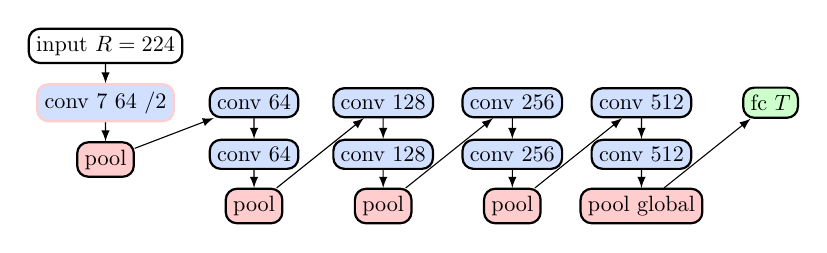
\begin{tikzpicture}[scale=0.82, every node/.style={scale=0.8}]
			\def \n {0.8}
			\def \s {2.0}
			\node[draw, rectangle, rounded corners, thick] at (-0.3, 0.1*\n) (in) {input $R=224$};
			\node[draw=xred, rectangle, rounded corners, thick, fill=xblue] at (-0.3, -1*\n) (conv1) {conv $7$ $64$ $/2$};
			\node[draw, rectangle, rounded corners, thick, fill=xred] at (-0.3, -2.1*\n) (pool1) {pool};
			\begin{scope}[on background layer]
				\draw[->, >=latex] (in) -- (conv1);
				\draw[->, >=latex] (conv1) -- (pool1);
			\end{scope}
			\node[draw, rectangle, rounded corners, thick, fill=xblue] at (\s, -1*\n) (conv3) {conv $64$};
			\node[draw, rectangle, rounded corners, thick, fill=xblue] at (\s, -2*\n) (conv4) {conv $64$};
			\node[draw, rectangle, rounded corners, thick, fill=xred] at (\s, -3*\n) (pool2) {pool};
			\begin{scope}[on background layer]
				\draw[->, >=latex] (pool1) -- (conv3);
				\draw[->, >=latex] (conv3) -- (conv4);
				\draw[->, >=latex] (conv4) -- (pool2);
			\end{scope}
			\node[draw, rectangle, rounded corners, thick, fill=xblue] at (2*\s, -1*\n) (conv5) {conv $128$};
			\node[draw, rectangle, rounded corners, thick, fill=xblue] at (2*\s, -2*\n) (conv6) {conv $128$};
			\node[draw, rectangle, rounded corners, thick, fill=xred] at (2*\s, -3*\n) (pool3) {pool};
			\begin{scope}[on background layer]
				\draw[->, >=latex] (pool2) -- (conv5);
				\draw[->, >=latex] (conv5) -- (conv6);
				\draw[->, >=latex] (conv6) -- (pool3);
			\end{scope}
			\node[draw, rectangle, rounded corners, thick, fill=xblue] at (3*\s, -1*\n) (conv8) {conv $256$};
			\node[draw, rectangle, rounded corners, thick, fill=xblue] at (3*\s, -2*\n) (conv9) {conv $256$};
			\node[draw, rectangle, rounded corners, thick, fill=xred] at (3*\s, -3*\n) (pool4) {pool};
			\begin{scope}[on background layer]
				\draw[->, >=latex] (pool3) -- (conv8);
				\draw[->, >=latex] (conv8) -- (conv9);
				\draw[->, >=latex] (conv9) -- (pool4);
			\end{scope}
			\node[draw, rectangle, rounded corners, thick, fill=xblue] at (4*\s, -1*\n) (conv11) {conv $512$};
			\node[draw, rectangle, rounded corners, thick, fill=xblue] at (4*\s, -2*\n) (conv12) {conv $512$};
			\node[draw, rectangle, rounded corners, thick, fill=xred] at (4*\s, -3*\n) (pool5) {pool global};
			\begin{scope}[on background layer]
				\draw[->, >=latex] (pool4) -- (conv11);
				\draw[->, >=latex] (conv11) -- (conv12);
				\draw[->, >=latex] (conv12) -- (pool5);
			\end{scope}
			\node[draw, rectangle, rounded corners, thick, fill=xgreen] at (5*\s, -1*\n) (fc1) {fc $T$};
			\begin{scope}[on background layer]
				\draw[->, >=latex] (pool5) -- (fc1);
			\end{scope}
		\end{tikzpicture}
	\end{center}

\end{frame}


\begin{frame}
	\frametitle{Modern Classification Networks}
	\framesubtitle{Training Deep Networks}

	Increasing depth is simple in theory
	\begin{itemize}
		\item Just add more conv layers between pooling layers
	\end{itemize}

	\bigskip

	In practice as a rule of thumb
	\begin{itemize}
		\item Increasing the depth like this improves performance
		\item With batch normalization and proper regularization
		\item Up to a depth of around $20$
	\end{itemize}

\end{frame}


\begin{frame}
	\frametitle{Modern Classification Networks}
	\framesubtitle{Training Deep Networks}

	Even deeper networks eventually perform worse
	\begin{itemize}
		\item Not intuitive (network could learn identity functions) %
		\item However doing so is challenging
	\end{itemize}

	\bigskip

	\begin{center}
		\copyrightbox[b]
		{\includegraphics[width=9cm]{images/deep-errors}}
		{\centering Image from [1]} %
	\end{center}

\end{frame}


\begin{frame}
	\frametitle{Modern Classification Networks}
	\framesubtitle{Residual Networks}

	\emph{Residual networks} (\emph{ResNets}) [1] facilitate this task
	\begin{itemize}
		\item Learn what to change about input
		\item Making it easy to learn identity function %
		\item By using \emph{skip-connections} and summation
	\end{itemize}

	\medskip

	\begin{center}
		\copyrightbox[b]
		{\includegraphics[width=5.2cm]{images/resnet-block}} %
		{\centering Image from [1]}
	\end{center}

\end{frame}


\begin{frame}
	\frametitle{Modern Classification Networks}
	\framesubtitle{Residual Networks}

	Idea is that
	\begin{itemize}
		\item Individual layers only change input a little
		\item But network has many more of them
	\end{itemize}

	\begin{center}
		\copyrightbox[b]
		{\includegraphics[width=3.3cm,angle=90]{images/resnet-34}}
		{\centering Image adapted from [1]}
	\end{center}

\end{frame}



\begin{frame}
	\frametitle{Modern Classification Networks}
	\framesubtitle{Residual Networks}

	Another benefit is easier gradient flow
	\begin{itemize}
		\item Recall that sum nodes propagate gradients without changes %
		\item And that gradients that join are summed %
	\end{itemize}

	\medskip

	\begin{center}
		\copyrightbox[b]
		{\includegraphics[width=5.2cm]{images/resnet-block}} %
		{\centering Image from [1]}
	\end{center}

\end{frame}


\begin{frame}
	\frametitle{Modern Classification Networks}
	\framesubtitle{Residual Networks}

	ResNet-34 ($R=224$)
	\begin{itemize}
		\item First and last layers identical to baseline design
	\end{itemize}

	\medskip

	\begin{center}
		\includegraphics[width=10cm]{images/resnet-34-graph}
	\end{center}

\end{frame}


\begin{frame}
	\frametitle{Modern Classification Networks}
	\framesubtitle{Residual Networks}

	Must support changes to $C,H,W$
	\begin{itemize}
		\item To enable pooling and adjusting feature map counts
	\end{itemize}

	\bigskip

	$1\times1$ (\emph{point-wise}) convolutions are a flexible tool
	\begin{itemize}
		\item Can adjust $C$ freely
		\item Can adjust $H,W$ via stride
	\end{itemize}

	\bigskip

	ResNet variant
	\begin{itemize}
		\item First $3\times3$ conv with stride 2 that doubles $C$
		\item Extra $1\times1$ conv with same configuration before sum
	\end{itemize}

\end{frame}


\begin{frame}
	\frametitle{Modern Classification Networks}
	\framesubtitle{Residual Networks}

	Such networks scale to depths of 1000 and more (!)
	\begin{itemize}
		\item $1202$ variant overfits below (training error $\approx0$)
	\end{itemize}

	\medskip

	\begin{center}
		\copyrightbox[b]
		{\includegraphics[width=5.5cm]{images/resnet-cifar-errors}}
		{\centering Image from [1]}
	\end{center}

\end{frame}


\begin{frame}
	\frametitle{Modern Classification Networks}
	\framesubtitle{Residual Networks}

	Very deep ResNets use more efficient blocks
	\begin{itemize}
		\item Reduce $C$ before expensive $3\times3$ conv (\emph{bottleneck layer})
	\end{itemize}

	\medskip

	\begin{center}
		\copyrightbox[b]
		{\includegraphics[width=4cm]{images/deep-resnet-block}}
		{\centering Image from [1]}
	\end{center}

\end{frame}


\begin{frame}
	\frametitle{Modern Classification Networks}
	\framesubtitle{Residual Networks}

	ResNets still perform great today
	\begin{itemize}
		\item Accuracy typically within $\approx 5\%$ of state of the art
		\item Good default architecture for deep networks
		\item PyTorch: \texttt{net = torchvision.models.resnet34()}
	\end{itemize}

	\bigskip
	Not optimized for efficiency though

\end{frame}


\begin{frame}
	\frametitle{Modern Classification Networks}
	\framesubtitle{Efficient Architectures}

	Efficiency usually matters
	\begin{itemize}
		\item More efficienct networks cost less to operate
		\item Hardware limitations (e.g.~mobile phones)
	\end{itemize}

	\bigskip

	We focus on efficiency during \emph{inference} (not training)
	\begin{itemize}
		\item In terms of accuracy vs.~FLOPS (or predictions/second)
	\end{itemize}

\end{frame}


\begin{frame}
	\frametitle{Modern Classification Networks}
	\framesubtitle{Efficient Architectures}

	Point-wise and \emph{depth-wise} convolutions are key ingredients %

	\smallskip

	\begin{center}
		\copyrightbox[b]
		{\includegraphics[width=7cm]{images/sep-conv}}
		{\centering Image from mc.ai}
	\end{center}

\end{frame}


\begin{frame}
	\frametitle{Modern Classification Networks}
	\framesubtitle{Efficient Architectures}

	Building blocks of MobileNet v2 [3]

	\medskip

	\begin{center}
		\copyrightbox[b]
		{\includegraphics[width=5cm]{images/mnet-v2.png}}
		{\centering Image from [2]}
	\end{center}

\end{frame}


\begin{frame}
	\frametitle{Modern Classification Networks}
	\framesubtitle{Efficient Architectures}


	\begin{center}
		\copyrightbox[b]
		{\includegraphics[width=7cm]{images/enet-perf.png}}
		{\centering Image from [3]}
	\end{center}

\end{frame}


\begin{frame}
	\frametitle{Modern Classification Networks}
	\framesubtitle{Network Scaling}

	We previously talked about varying the depth of our networks

	\bigskip
	This is a form of \emph{network scaling}
	\begin{itemize}
		\item Adapt capacity of network
		\item To optimize performance given task at hand
		\item While considering the computational budget
	\end{itemize}

	\bigskip
	We will next cover other forms

\end{frame}


\begin{frame}
	\frametitle{Modern Classification Networks}
	\framesubtitle{Network Scaling}

	\begin{center}
		\copyrightbox[b]
		{\includegraphics[width=10cm]{images/net-scaling}}
		{\centering Image from [3]}
	\end{center}

\end{frame}


\begin{frame}
	\frametitle{Modern Classification Networks}
	\framesubtitle{Network Scaling}

	Scaling width, depth, and resolution are all effective
	\begin{itemize}
		\item Impact on FLOPS varies (depends on architecture)
		\item Improvements compound (with diminishing returns)
	\end{itemize}

	\bigskip

	\begin{center}
		\copyrightbox[b]
		{\includegraphics[width=10cm]{images/net-scaling-imagenet}}
		{\centering Scaling by width, depth, resolution, in this order. Image from [3].}
	\end{center}

\end{frame}


\begin{frame}
	\frametitle{Modern Classification Networks}
	\framesubtitle{Network Scaling}

	Given all this, how can we design efficient networks?

	\bigskip
	For practicioners like you
	\begin{itemize}
		\item Stick to established architectures that work well
		\item ResNet, EfficientNet, ConvNeXt are examples
	\end{itemize}

	\bigskip
	For researchers in the field
	\begin{itemize}
		\item Manually via trial and error (based on prior work)
		\item Automatically via \emph{neural architecture search} (\emph{NAS}) %
	\end{itemize}

\end{frame}


\begin{frame}
	\frametitle{Modern Classification Networks}
	\framesubtitle{ConvNeXt}

	State of the art architecture
	\begin{itemize}
		\item Design inspired by Transformers (later)
	\end{itemize}

	\medskip

	\begin{center}
		\copyrightbox[b]
		{\includegraphics[width=7cm]{images/convnext-perf.png}}
		{\centering Image from [5]}
	\end{center}

\end{frame}


\begin{frame}
	\frametitle{Modern Classification Networks}
	\framesubtitle{ConvNeXt}



	\begin{center}
		\copyrightbox[b]
		{\includegraphics[width=5cm]{images/convnext-block.png}}
		{\centering Image from [5]}
	\end{center}

\end{frame}


\begin{frame}
	\frametitle{Modern Classification Networks}
	\framesubtitle{ConvNeXt}

	\begin{center}
		\copyrightbox[b]
		{\includegraphics[width=5cm]{images/convnext-deriv.png}}
		{\centering Image from [5]}
	\end{center}

\end{frame}


{
\setbeamertemplate{footline}{}
\begin{frame}

	\begin{tikzpicture}[remember picture,overlay]
		\fill[white] (current page.north west) rectangle (current page.south east);
	\end{tikzpicture}

	\begin{center}
		\textcolor[rgb]{0.9,0.9,0.9}{blank page}
	\end{center}

\end{frame}
}


\begin{frame}
	\frametitle{Pushing Classification Performance}
	\framesubtitle{Fine-Tuning}

	Data augmentation \& regularization cannot replace data
	\begin{itemize}
		\item Deep learning scales extremely well with data
		\item So obtaining more data should be a priority
	\end{itemize}

	\bigskip

	For this reason, a powerful technique is \emph{fine-tuning}
	\begin{itemize}
		\item \emph{Pre-train} network on related large dataset (e.g.~ImageNet)
		\item Then fine-tune same network on smaller target dataset
	\end{itemize}

	\bigskip

	Idea is to exploit information present in both datasets


\end{frame}



\begin{frame}
	\frametitle{Pushing Classification Performance}
	\framesubtitle{Fine-Tuning}

	For instance we could
	\begin{itemize}
		\item Pre-train a network on ImageNet ($1000$ classes)
		\item Then replace its linear classifier with one for $2$ classes
		\item And fine-tune the network on our cats vs.~dogs dataset
	\end{itemize}

	\bigskip

	Fine-tuning almost always helps
	\begin{itemize}
		\item Even if target dataset is large itself %
		\item Assuming both datasets are related (the more, the better)
	\end{itemize}

\end{frame}


\begin{frame}
	\frametitle{Pushing Classification Performance}
	\framesubtitle{Fine-Tuning}

	If the target dataset is very small
	\begin{itemize}
		\item Consider fine-tuning just the new classifier
		\item Can be done by freezing parameters of other layers
	\end{itemize}

	\bigskip

	If not, a good strategy is to
	\begin{itemize}
		\item First fine-tune only new classifier %
		\item Then unfreeze other layers and train some more
		\item Using a larger learning rate for classifier than for rest
	\end{itemize}

\end{frame}


\begin{frame}
	\frametitle{Pushing Classification Performance}
	\framesubtitle{Handling Imbalanced Data}

	So far we have assumed balanced data
	\begin{itemize}
		\item Same number of samples per class
	\end{itemize}

	\bigskip

	If this is not the case
	\begin{itemize}
		\item Classifier will pay more attention to majority classes
		\item Leading to bad accuracy for minority classes
	\end{itemize}

	\bigskip

	This is usually not desired and must be addressed
	\begin{itemize}
		\item We will cover two popular options
	\end{itemize}
\end{frame}


\begin{frame}
	\frametitle{Pushing Classification Performance}
	\framesubtitle{Handling Imbalanced Data}

	Via \emph{class weights} on the loss
	\begin{itemize}
		\item Multiply per-sample losses by weights
		\item With weights based on inverse class frequencies
		\item Easy to implement and no computational overhead
	\end{itemize}

	\bigskip

	Via \emph{oversampling} of the training data
	\begin{itemize}
		\item Draw samples with replacement to balance class frequencies
		\item Works well in combination with data augmentation
		\item Considerable computational overhead
	\end{itemize}

\end{frame}


\begin{frame}
	\frametitle{Remarks}

	We will now move on from classification to other tasks
	\begin{itemize}
		\item Most architectures use a classification network as \emph{backbone} %
		\item Train a classification network on large dataset (e.g.~ImageNet)
		\item Adapt network for e.g. object detection
	\end{itemize}

	\bigskip

	This is a form of \emph{transfer learning}
	\begin{itemize}
		\item Adapt a model trained on one task to perform well on another %
	\end{itemize}

\end{frame}


\renewcommand\emph[1]{\oldemph{#1}}

\begin{frame}
	\frametitle{Bibliography}

	[1] He et al.~Deep Residual Learning for Image Recognition.~2015 \\\medskip
	[2] Sandler et al.~MobileNetV2.~2018 \\\medskip
	[3] Tan~\&~Le.EfficientNet.~2019 \\\medskip
	[4] Srivastava et al.~Dropout.~2014 \\\medskip
	[5] Liu et al.~A ConvNet for the 2020s.~2022

\end{frame}


\end{document}
